% Options for packages loaded elsewhere
\PassOptionsToPackage{unicode}{hyperref}
\PassOptionsToPackage{hyphens}{url}
\documentclass[
  11pt,
  a4paper,
]{article}
\usepackage{xcolor}
\usepackage[margin=22mm]{geometry}
\usepackage{amsmath,amssymb}
\setcounter{secnumdepth}{-\maxdimen} % remove section numbering
\usepackage{iftex}
\ifPDFTeX
  \usepackage[T1]{fontenc}
  \usepackage[utf8]{inputenc}
  \usepackage{textcomp} % provide euro and other symbols
\else % if luatex or xetex
  \usepackage{unicode-math} % this also loads fontspec
  \defaultfontfeatures{Scale=MatchLowercase}
  \defaultfontfeatures[\rmfamily]{Ligatures=TeX,Scale=1}
\fi
\usepackage{lmodern}
\ifPDFTeX\else
  % xetex/luatex font selection
\fi
% Use upquote if available, for straight quotes in verbatim environments
\IfFileExists{upquote.sty}{\usepackage{upquote}}{}
\IfFileExists{microtype.sty}{% use microtype if available
  \usepackage[]{microtype}
  \UseMicrotypeSet[protrusion]{basicmath} % disable protrusion for tt fonts
}{}
\makeatletter
\@ifundefined{KOMAClassName}{% if non-KOMA class
  \IfFileExists{parskip.sty}{%
    \usepackage{parskip}
  }{% else
    \setlength{\parindent}{0pt}
    \setlength{\parskip}{6pt plus 2pt minus 1pt}}
}{% if KOMA class
  \KOMAoptions{parskip=half}}
\makeatother
\usepackage{graphicx}
\makeatletter
\newsavebox\pandoc@box
\newcommand*\pandocbounded[1]{% scales image to fit in text height/width
  \sbox\pandoc@box{#1}%
  \Gscale@div\@tempa{\textheight}{\dimexpr\ht\pandoc@box+\dp\pandoc@box\relax}%
  \Gscale@div\@tempb{\linewidth}{\wd\pandoc@box}%
  \ifdim\@tempb\p@<\@tempa\p@\let\@tempa\@tempb\fi% select the smaller of both
  \ifdim\@tempa\p@<\p@\scalebox{\@tempa}{\usebox\pandoc@box}%
  \else\usebox{\pandoc@box}%
  \fi%
}
% Set default figure placement to htbp
\def\fps@figure{htbp}
\makeatother
\setlength{\emergencystretch}{3em} % prevent overfull lines
\providecommand{\tightlist}{%
  \setlength{\itemsep}{0pt}\setlength{\parskip}{0pt}}
\usepackage{bookmark}
\IfFileExists{xurl.sty}{\usepackage{xurl}}{} % add URL line breaks if available
\urlstyle{same}
\hypersetup{
  pdftitle={Towards abc I: the theorems of Stewart and Tijdeman},
  pdfauthor={GPT-6 Astra (OpenAI), Ultra},
  hidelinks,
  pdfcreator={LaTeX via pandoc}}

\title{Towards abc I: the theorems of Stewart and Tijdeman}
\author{GPT-6 Astra (OpenAI), Ultra}
\date{October 2026}

\providecommand{\Eta}{\mathrm{H}}
\begin{document}
\maketitle

\emph{Written by GPT-6 Astra (OpenAI) in Codex, Ultra setting, October
2026. Self-checked by the writing AI. Public domain (CC0).}

A large integer can be built from small prime powers. The equation
\(a+b=c\) asks how far this can happen to three pairwise coprime
integers at the same time. Its natural measure of prime support is
\(G=\operatorname{rad}(abc)\).

Oesterlé's fixed-power question asks whether an absolute exponent can
bound \(c\) by a power of \(G\). The abc conjecture asks more precisely:
for every \(\epsilon>0\), does a constant \(C_\epsilon\) exist such that
\[
 c\le C_\epsilon G^{1+\epsilon}
\] for every positive coprime triple? Oesterlé's
\href{https://www.numdam.org/article/SB_1987-1988__30__165_0.pdf}{Section
3, Conjecture 3} uses three nonzero integers with sum zero; moving the
negative entry to the other side gives this positive form. The
equivalence with the formulation \(c^{1-\epsilon}\le C'_\epsilon G\),
including the change of constants, is proved in
\href{../the-field-with-one-element/the-projective-line-over-f-1-and-the-abc-conjecture.html\#section-5.2}{the
F1 course, Lemma 5.5}. Its
\href{../the-field-with-one-element/the-projective-line-over-f-1-and-the-abc-conjecture.html\#section-5.3}{Section
5.3} proves the relation with Smirnov's conjectural Hurwitz inequality.
Those equivalences are not repeated here.

This lesson proves two statements that lie on opposite sides of the
question. First, the factor \(G\) alone, even multiplied by one absolute
constant, is insufficient: Stewart and Tijdeman construct infinitely
many triples with \(c/G\) exponentially large in
\(\sqrt{\log G}/\log\log G\). Second, p-adic linear forms give an
effective bound \(\log c<G^{1+o(1)}\), with all constants made explicit
below. The logarithm on the left is crucial: this is still much weaker
than the conjectural bound for \(c\) itself.

The lower bound uses the quantitative prime number theorem proved in
NT-ZETA. Its counting and congruence arguments are elementary and are
developed first. The upper bound uses Lesson 10's complete p-adic
estimate, with independent prime bases, the case at two, and the
inversion of the coefficient bound all made explicit. The final section
translates these results into the defect notation of the F1 lesson.

\subsection{1. Three estimates for the first odd
primes}\label{three-estimates-for-the-first-odd-primes}

We use \(a+b=c\), with \(a,b,c\) positive and pairwise coprime, and
write \[
 G=\operatorname{rad}(abc)=\prod_{p\mid abc}p.
 \tag{19.1}
\] The radical remembers each prime once and forgets its exponent. The
lower-bound construction will produce a large power of two in one
summand while using a controlled set of odd primes in the other two.

The construction is due to
\href{https://uwaterloo.ca/pure-mathematics/sites/default/files/uploads/documents/log_0023.pdf}{Stewart
and Tijdeman, \emph{On the Oesterlé--Masser conjecture}, Theorem 2}. We
prove the counting and congruence steps below, using the programme proof
of the quantitative prime number theorem.

Let \(p_1=3,p_2=5,\ldots\) be the odd primes in increasing order, and
put \(P_r=\prod_{j=1}^r p_j\).

\textbf{Lemma 19.1.} As \(r\to\infty\), \[
 \begin{aligned}
 p_r&=r(\log r+\log\log r-1+o(1)),\\
 \log P_r&=r(\log r+\log\log r-1+o(1)),\\
 \sum_{j=1}^r\log\log p_j&\le r(\log\log r+o(1)).
 \end{aligned}
 \tag{19.2}
\] In particular, given \(\epsilon>0\), each \(o(1)\) on the right can
be replaced by \(\epsilon\) in an upper bound for all sufficiently large
\(r\).

\textbf{Proof.} The programme theorem
\href{../NT-ZETA/NT-ZETA-12.html}{\emph{The prime number theorem with
the classical error term}, Theorem 2.1} proves both
\(\theta(x)=x+O(xe^{-c\sqrt{\log x}})\) and
\(\pi(x)=\operatorname{li}(x)+O(xe^{-c\sqrt{\log x}})\), with an
absolute positive \(c\). The exponential error is \(O(x/\log^3x)\): for
\(v=\sqrt{\log x}\), the function \(v^6e^{-cv}\) is bounded. Two
integrations by parts give \[
 \pi(x)=\frac{x}{\log x}+\frac{x}{\log^2x}
             +O\left(\frac{x}{\log^3x}\right).
 \tag{19.3}
\] For the integral remainder, split at \(\sqrt x\). The lower part is
\(O(\sqrt x)\); on the upper part, \((\log t)^{-3}\le8(\log x)^{-3}\).
This also accounts for the fixed lower-endpoint constants.

Since \(\pi(p_r)=r+1\), (19.3) first yields \(p_r\sim r\log r\), by the
logarithmic inversion proved in
\href{../NT-ZETA/NT-ZETA-09.html}{\emph{The prime number theorem},
Corollary 3.2}. Write \(L=\log r\) and \(l=\log L\). Inverting (19.3)
once gives \[
 \frac{p_r}{r}=\log p_r-1+O(1/\log p_r).
 \tag{19.4}
\] Replacing \(r+1\) by \(r\) changes the right side by
\(O(\log p_r/r)\), which is absorbed in the error. The first asymptotic
gives \(\log p_r=L+l+o(1)\), so (19.4) proves the first line of (19.2).
Next, \(\log P_r=\theta(p_r)-\log2=p_r+o(r)\): the exponential error
divided by \(r\) tends to zero because \(p_r/r\asymp\log r\). This
proves the second line. Finally monotonicity gives \[
 \sum_{j=1}^r\log\log p_j\le r\log\log p_r
       =r(\log\log r+o(1)),
\] which is the last assertion. \(\square\)

The constant minus one in the first two lines matters. Losing it would
lose part of the exponential gain in the final construction.

\subsection{2. Counting integers with prescribed prime
divisors}\label{counting-integers-with-prescribed-prime-divisors}

For distinct primes \(q_1,\ldots,q_r\), let \(N(X)\) be the number of
positive integers at most \(X>1\) whose prime divisors belong to this
set. The integer one is included.

\textbf{Lemma 19.2 (simplex count).} For every such \(X\), \[
 N(X)\ge\frac{(\log X)^r}{r!\prod_{j=1}^r\log q_j}.
 \tag{19.5}
\] For the first \(r\) odd primes and any \(\epsilon>0\), all
sufficiently large \(r\) satisfy, uniformly for \(X>1\), \[
 N(X)>\left(\frac{e^{1-2\epsilon}\log X}
                          {r\log r}\right)^r.
 \tag{19.6}
\]

\textbf{Proof.} Unique factorization identifies these integers with
vectors \(n\in\mathbb Z_{\ge0}^r\) satisfying
\(\sum_jn_j\log q_j\le\log X\). Consider the real simplex \[
 T=\left\{u_j\ge0:\ \sum_ju_j\log q_j\le\log X\right\}.
 \tag{19.7}
\] For every point \(u\in T\), its coordinatewise floor is an admissible
integer vector. Hence the half-open unit cubes based at the admissible
vectors cover \(T\); their interiors are disjoint. Their total volume is
\(N(X)\).

For completeness, the simplex \(v_j\ge0\), \(\sum v_j\le L\) has volume
\(L^r/r!\). Induction begins with length \(L\); integrating the last
coordinate gives \(\int_0^L(L-t)^{r-1}/(r-1)!\,dt=L^r/r!\). The diagonal
change of variables \(v_j=u_j\log q_j\) has Jacobian
\(\prod_j\log q_j\), proving (19.5).

Monotonicity of \(\log t\) bounds the sum \(\log(r!)\) between
\(\int_1^r\log t\,dt\) and that integral plus \(\log r\). Thus
\(\log(r!)=r\log r-r+O(\log r)\). Use this and the last line of Lemma
19.1 in the logarithm of (19.5). For sufficiently large \(r\), \[
 \log(r!)+\sum_{j=1}^r\log\log p_j
 <r(\log r+\log\log r-1+2\epsilon).
\] Exponentiation proves (19.6). The threshold depends on \(\epsilon\),
not on \(X\). \(\square\)

\subsection{3. Turning a congruence into a small
radical}\label{turning-a-congruence-into-a-small-radical}

\textbf{Lemma 19.3 (the two-adic box argument).} Suppose \(S\) is a set
of \(N\ge2\) distinct positive odd integers at most \(X\), all supported
on a set of primes with product \(P\). There is a coprime triple
\(a+b=c\), with \(c\le X\), such that \[
 G<\frac{4Pc}{N},\qquad
 v_2(b)\ge\left\lfloor\log_2(N-1)\right\rfloor.
 \tag{19.8}
\]

\textbf{Proof.} Set \(m=\lfloor\log_2(N-1)\rfloor\). Then
\(2^m<N\le2^{m+1}\). Among the \(N\) integers, two, say \(x>y\), have
the same residue modulo \(2^m\). Let \(g=\gcd(x,y)\), and put \[
 a=y/g,\qquad b=(x-y)/g,\qquad c=x/g.
 \tag{19.9}
\] These are positive and \(a+b=c\). Any common divisor of two would
divide both \(x/g\) and \(y/g\), so the triple is pairwise coprime.
Since \(g\) is odd, \(v_2(b)=v_2(x-y)\ge m\); dividing by the common
divisor does not remove the large power of two.

Both \(a,c\) are odd and supported on the prescribed primes. Write
\(b=2^vu\), with \(u\) odd and \(v\ge1\). Since
\(\operatorname{rad}(u)\le u\), \[
 G\le P\operatorname{rad}(b)
   \le\frac{2Pb}{2^v}<\frac{2Pc}{2^m}
   \le\frac{4Pc}{N}.
 \tag{19.10}
\] The strict inequality uses \(b<c\). This also proves \(c\le x\le X\)
and all assertions. \(\square\)

\begin{minipage}[t]{\linewidth}
\centering
\pandocbounded{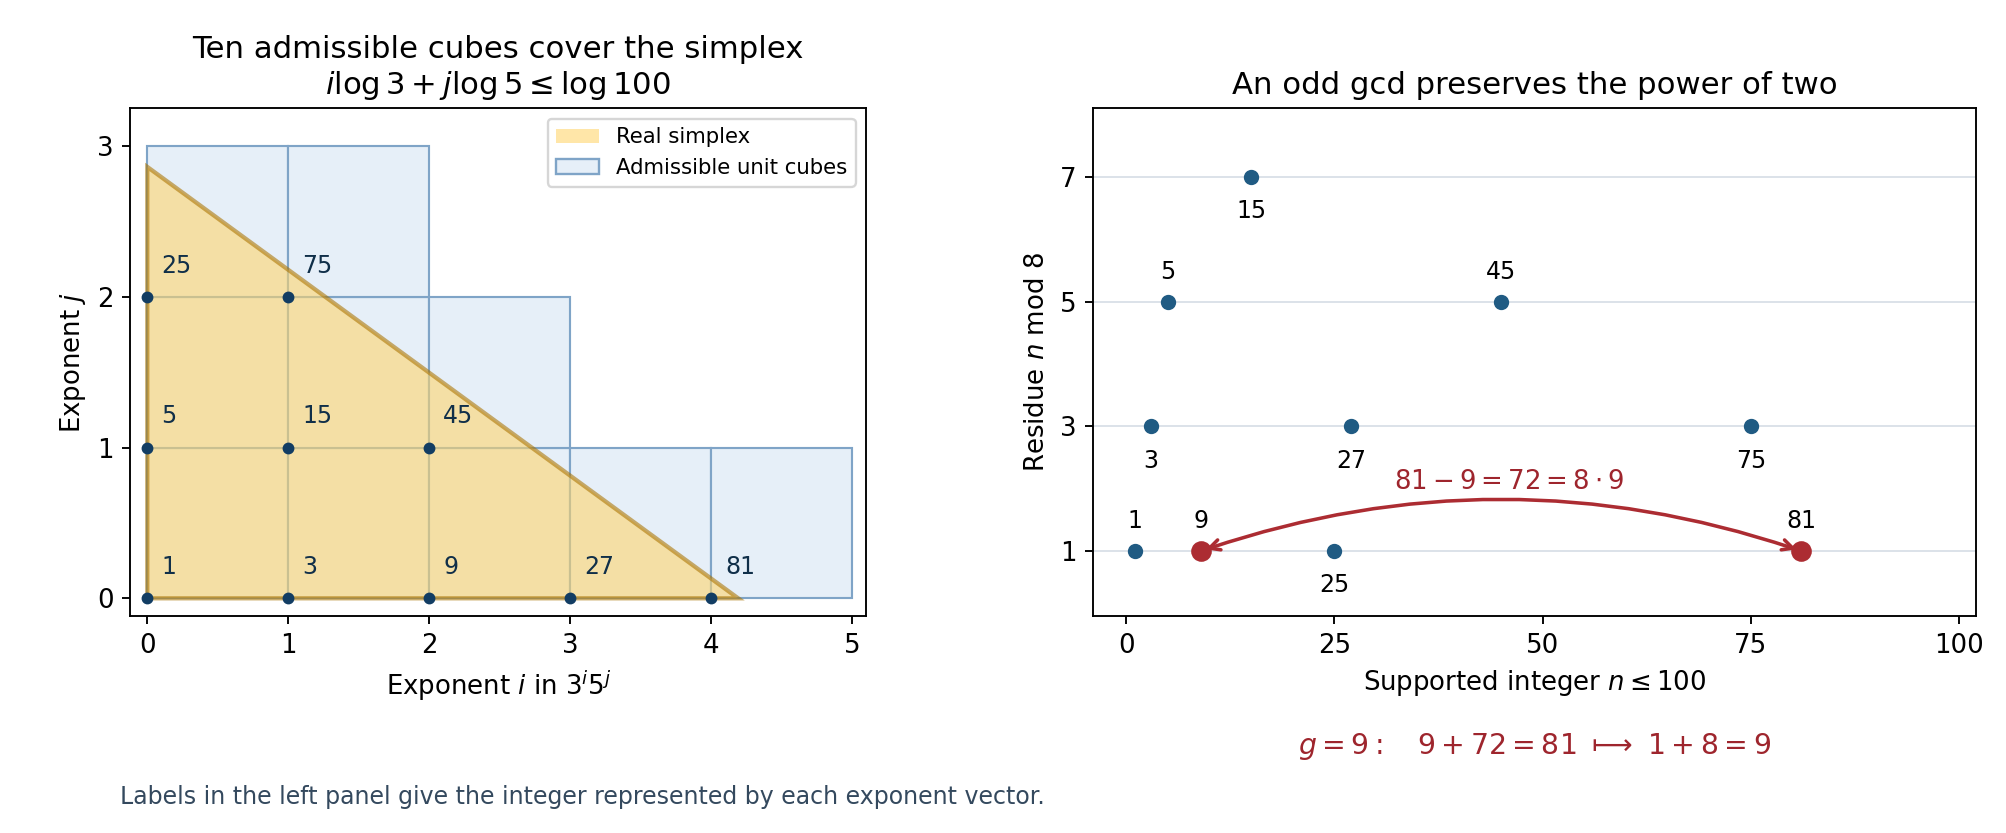
\includegraphics[keepaspectratio,alt={A simplex covered by ten unit cubes, and the ten supported integers sorted by their residues modulo eight.}]{../figures/abc-construction.png}}
\par\smallskip
\begin{flushleft}\small
\emph{Figure 19.1. With primes 3 and 5 and \(X=100\), the ten admissible
exponent vectors cover the simplex by their unit cubes, as in Lemma
19.2. The labels give \(3^i5^j\). Here \(N=10\) and
\(m=\lfloor\log_2(N-1)\rfloor=3\). The integers 9 and 81 occupy the same
residue class modulo eight. Their common divisor is nine, so division
gives \(1+8=9\) and preserves the valuation three of the difference at
two. The radical is six and satisfies \(6<4\cdot15\cdot9/10=54\), as in
Lemma 19.3. This finite example illustrates the counting and valuation
mechanisms; infinitude is proved in Theorem 19.4. Human-source
background: Stewart and Tijdeman, Lemma 3 and the proof of Theorem 2.
\href{figure_sources/abc-construction.py}{Reproducible figure
program}.}
\end{flushleft}
\end{minipage}\par\medskip


\subsection{4. The Stewart--Tijdeman lower
bound}\label{the-stewarttijdeman-lower-bound}

\textbf{Theorem 19.4.} For every \(\delta>0\), infinitely many coprime
positive triples \(a+b=c\) satisfy \[
 c>G\exp\left((4-\delta)
                    \frac{\sqrt{\log G}}{\log\log G}\right).
 \tag{19.11}
\]

\textbf{Proof.} It suffices to prove the assertion for \(0<\delta\le1\),
since decreasing \(\delta\) strengthens the inequality for \(G\ge6\).
Put \(\epsilon=\delta/16\). For large integers \(r\), set \[
 X=\exp((r\log r)^2),
 \qquad S=\left\{n\le X:\ p\mid n\Longrightarrow
                       p\in\{p_1,\ldots,p_r\}\right\}.
 \tag{19.12}
\] Lemmas 19.1--19.2 give \[
 \log P_r<r(\log r+\log\log r-1+\epsilon),\qquad
 \log|S|>r(\log r+\log\log r+1-2\epsilon).
 \tag{19.13}
\] Apply Lemma 19.3 to \(S\). If \(r\) is large enough that
\(\log4<\epsilon r\), its coprime triple satisfies \[
 \log(c/G)>\log|S|-\log P_r-\log4
                  >(2-4\epsilon)r.
 \tag{19.14}
\] In particular \(G<c\le X\). Also \(G\ge6\): the positive even integer
\(b\) contributes two, and the odd integer \(c>1\) contributes an odd
prime.

To replace \(X\) by the actual radical, put
\(f(t)=\sqrt{\log t}/\log\log t\) for \(t\ge6\). Writing \(u=\log t\),
differentiation shows that \(\sqrt u/\log u\) increases when
\(\log u>2\). On the fixed interval \([6,e^{e^2}]\) it is bounded. Since
\(f(X)\to\infty\), for all large \(r\) we have \(f(t)\le f(X)\)
throughout \(6\le t\le X\): use that fixed bound below \(e^{e^2}\) and
monotonicity above it. Moreover the chosen value of \(X\) gives the
exact inequality \[
 f(X)=\frac{r\log r}{2(\log r+\log\log r)}<\frac r2.
 \tag{19.15}
\] Thus \[
 (4-\delta)f(G)<(2-\delta/2)r
       <(2-4\epsilon)r<\log(c/G),
\] which proves (19.11).

Finally \(|S|\to\infty\) by (19.13). The valuations \(v_2(b)\) in Lemma
19.3 therefore tend to infinity. Since a fixed positive integer has a
finite two-adic valuation, the constructed coprime triples cannot belong
to a finite set. This proves the required infinitude, including the
effect of the division by \(g\). \(\square\)

The constant four has two sources: the count of admissible integers
exceeds the prime product by \(e^{(2-o(1))r}\), and
\(\sqrt{\log X}/\log\log X\sim r/2\). The argument proves that a fixed
constant multiple of \(G\) cannot bound all \(c\). It does not
contradict a bound \(C_\eta G^{1+\eta}\) for each fixed \(\eta>0\).

\subsection{5. The elementary cost of a set of
primes}\label{the-elementary-cost-of-a-set-of-primes}

We now turn to an upper bound. Write \(L=\log G\), and, for \(G\ge6\),
put \[
 \Psi(G)=\frac{L\log\log(L+\log8)}{\log L}.
 \tag{19.16}
\] Thus \(\Psi(G)=\log G\log\log\log(8G)/\log\log G\). The shift by
eight makes the numerator positive. In particular, \(\Psi(G)=o(\log G)\)
as \(G\to\infty\).

\textbf{Lemma 19.5 (prime products and logarithmic products).} Let
\(G\ge6\) be squarefree, with \(r\) prime factors. Then \(r!\le G\). If
\(L\ge e^6\), then \[
 r\le\frac{2L}{\log L},\qquad
 \log\max\left\{1,\prod_{q\in T}\log q\right\}
       \le2\Psi(G)
 \tag{19.17}
\] for every nonempty subset \(T\) of its prime factors. For every
\(G\ge6\), \[
 \frac12<\Psi(G)\le L,\qquad \log L\le4\Psi(G).
 \tag{19.18}
\]

\textbf{Proof.} In increasing order the distinct prime factors are at
least \(2,3,\ldots,r+1\); their product is at least \(r!\). The integral
bound \(\log(r!)\ge r\log r-r+1\) follows by summing the integrals of
the increasing function \(\log x\) over the intervals \([j,j+1]\).

Put \(z=\log L\ge6\). If \(r>2L/z\), then \[
 \log r-1>z-\log z+\log2-1>z/2.
\] For the last inequality, the function \(z/2-\log z+\log2-1\)
increases for \(z>2\) and is positive at four. Consequently
\(\log(r!)>L\), a contradiction. This proves the rank bound.

If \(m=|T|\), the arithmetic--geometric mean inequality gives
\(\prod_{q\in T}\log q\le(L/m)^m\). To verify the inequality here, let
\(A\) be the mean of the positive numbers \(\log q\). The function
\(x-1-\log x\) has minimum zero at one. Sum
\(\log((\log q)/A)\le(\log q)/A-1\) over the \(m\) primes, and use
\(A\le L/m\). The function \(x\log(L/x)\) increases for \(0<x<L/e\).
Since \(m\le r\le2L/z<L/e\), \[
 \log\prod_{q\in T}\log q
 \le\frac{2L}{z}\log(z/2)
 \le\frac{2L\log z}{z}\le2\Psi(G).
\] The right side is positive, so the same bound applies after taking
the maximum with one.

Here are useful bounds also covering the small values of \(G\). For
\(L\ge\log6\), \(\log\log(L+\log8)>1/4\). Indeed \(\log48>15/4\),
\(\log(15/4)>13/10\), and \(\log(13/10)>1/4\). These three numerical
inequalities follow, respectively, from \(e^{15/4}<48\),
\(e^{13/10}<15/4\), and \(e^{1/4}<13/10\); the positive exponential
series proves each, with its tail bounded by a geometric series. Since
\(L/\log L\ge e>2\) for \(L>1\), the first bound in (19.18) follows.
Next \(\log(L+\log8)\le L\): the function \(e^L-L\) increases on this
range, and \(6-\log6>\log8\). Taking logarithms proves \(\Psi(G)\le L\).
Finally \((\log L)^2\le L\), because the maximum of \(z^2e^{-z}\), for
\(z>0\), is \(4/e^2<1\). Combine this with \(\Psi(G)>L/(4\log L)\) to
obtain the last bound. \(\square\)

The logarithmic product in this lemma has logarithm
\(O(\log G\log\log\log G/\log\log G)\). Keeping this smaller term,
rather than bounding every logarithm by \(G\), is essential for the
exponent tending to one.

\subsection{6. Applying the proved p-adic
estimate}\label{applying-the-proved-p-adic-estimate}

We use \href{TR-BAKER-10.html}{Lesson 10, Theorem 10.154}, including
its rank-one case. Its complete proof is in that lesson; no external
estimate is being substituted for it. For independent local units
\(\alpha_1,\ldots,\alpha_n\) in a number field of degree \(d\), write
\(t=f\log p\), \(\Omega=\prod h(\alpha_j)\), and
\(B\ge\max\{3,|b_1|,\ldots,|b_n|\}\). The estimate is \[
 \operatorname{ord}_{\mathfrak p}
       (\alpha_1^{b_1}\cdots\alpha_n^{b_n}-1)
 < C_1^*\Omega\max\{\log B,t\}.
 \tag{19.19}
\] For the fields used here, \(\max\{1,\log d\}=1\), and the exact
constant (10.449) gives \[
 C_1^*=
 c_0\mathfrak a^n
 \frac{n^n(n+1)^{n+2}d^{n+2}}{n!q^ut}
 \max\left\{\frac{p^f}{\delta t^{n+1}},
                         \frac{e^n}{n^n}\right\}A_n,
 \quad A_n=\max\{4+\log((n+1)d),1,t\}.
 \tag{19.20}
\] Here \(\delta\ge1\) is the saturated residue index, \(q^u\ge1\) is
the indicated root-of-unity order, and \(e=\exp(1)\) in this formula.
The local ramification index in our applications is one. The proved
table in Lemma 10.151 permits \(c_0\le2680\), and \(\mathfrak a\le26\).
We keep a parameter \(C_0\ge\max\{1,c_0\}\), so the dependence on the
input constant will be visible.

\textbf{Lemma 19.6 (a radical bound retaining the logarithm of the
height).} Let \(a+b=c\) be a pairwise coprime positive triple other than
\((1,1,2)\). Put \(Q=\log c\), \(L=\log G\), \(r=\omega(G)\), and
\(n=r-1\). There is a prime \(p\mid G\) such that, with \[
 \Omega=\prod_{q\mid G,\ q\ne p}\log q,
 \qquad
 E=200C_0\,400^n(n+1)^2GL^2\max\{1,\Omega\},
 \tag{19.21}
\] one has \[
 Q<E(4L+\log Q),\qquad
 Q<2E\bigl(4L+\log(2E)\bigr).
 \tag{19.22}
\]

\textbf{Proof.} Except for \((1,1,2)\), the radical is at least six. To
see this, precisely one of \(a,b,c\) is even. If two were even they
would have a common factor; if all were odd their sum relation would
fail. If no odd prime occurred, the two odd entries would both be one,
giving the exceptional triple. Thus \(r\ge2\), \(n\ge1\), and \(c\ge3\).

Let \(\beta=\max_{q\mid abc}v_q(abc)\), and choose a prime \(p\)
attaining it. Pairwise coprimality puts this prime in precisely one of
the three entries. Use the rational number \[
 \Xi=\begin{cases}
 (c/b)^2,&p\mid a,\\
 (c/a)^2,&p\mid b,\\
 (a/b)^2,&p\mid c.
 \end{cases}
 \tag{19.23}
\] All denominators are p-adic units. Factoring the difference of the
two squares proves \(v_p(\Xi-1)\ge\beta\). In the last case \(a\ne b\),
since equality and coprimality would give the excluded triple. Thus
\(\Xi\ne1\) in all cases. Squaring avoids introducing a torsion sign
base.

Take as bases all \(n\) distinct primes dividing \(G/p\). They are
multiplicatively independent: the valuation at each of these rational
primes forces its exponent in any relation to vanish. Expressing (19.23)
in these bases gives integer coefficients of absolute value at most
\(2\beta\); some may be zero, which (19.19) allows. Their absolute
logarithmic heights are \(\log q\).

For odd \(p\), use \(K=\mathbb Q\), so \(d=f=1\). At two use
\(K=\mathbb Q(\zeta_3)\). The polynomial \(X^2+X+1\) is irreducible
modulo two. The discriminant of \(1,\zeta_3\) is \(-3\). Its index in
the full ring of integers has square dividing three, by the determinant
change-of-basis formula for discriminants; that index is therefore one.
The integral basis \(1,\zeta_3\) therefore gives the residue field
\(\mathbb F_4\) and ramification index one. Equivalently, the quotient
of its ring of integers by two is the field
\(\mathbb F_2[X]/(X^2+X+1)\). Thus \(d=f=2\), and the valuation of a
rational number at this prime is still \(v_2\). These are exactly the
odd-prime cases and case V allowed in Theorem 10.154. Uniformly,
\(d\le2\), \(t>1\), and \(p^f\le2p\).

The integral factorial bound gives \(n!\ge(n/e)^n\), and
\((1+1/n)^n<e\). Also \(p\,n!\le G\), since the other \(n\) primes have
product at least \(n!\). Apply these facts directly to (19.20), first
replacing its maximum by a sum: \[
 \begin{aligned}
 C_1^*
 &\le4C_0\,52^n\frac{(n+1)^{n+2}}{n!}
                    (2pn^n+e^n)A_n\\
 &<12eC_0(52e^2)^n(n+1)^2GA_n\\
 &<40C_0\,400^n(n+1)^2GA_n.
 \end{aligned}
 \tag{19.24}
\] Indeed \(pn^n\le e^nG\), and \(e^n\le e^nG\). The last line uses
\(e<11/4\), so \(52e^2<400\) and \(12e<40\). This is the cancellation of
the rank factor against the radical; it does not require \(p\) to be the
largest prime.

Since \(r\log2\le L\), \(\log(2r)\le r<2L\) for \(r\ge2\), and \(4<3L\),
we have \(A_n\le5L\). Also \(t\le2L\). Every entry of the triple is at
most \(c\), so \(\beta\le Q/\log2\) and \(Q>1\). Choose
\(B=\max\{3,2\beta\}\le3Q/\log2\). Then
\(\max\{\log B,t\}\le\log Q+4L\), using \(\log(3/\log2)<2<2L\). The
estimate (19.19) yields \[
 \beta<200C_0\,400^n(n+1)^2GL\Omega(\log Q+4L).
\] Finally \(Q\le\beta L\), by the prime factorization of \(c\).
Enlarging \(\Omega\) to \(\max\{1,\Omega\}\) proves the first inequality
of (19.22).

For the second, put \(A=4L+\log(2E)>1\). If \(Q\ge2EA\), then
\(x=Q/(2E)\ge A\), while the first inequality would say \(2x<A+\log x\).
But \(\log x\le x-1\) implies \(A+\log x\le2x-1\), a contradiction.
\(\square\)

\subsection{7. An upper exponent tending to
one}\label{an-upper-exponent-tending-to-one}

\textbf{Theorem 19.7.} With the p-adic constant bounded by \(C_0\ge1\)
as above, define \[
 K=10400+2\log(200C_0),\qquad
 \kappa=K+4+2\log\bigl(2(K+6)\bigr).
 \tag{19.25}
\] Every coprime positive triple \(a+b=c\) with \(G\ge6\) satisfies \[
 \log c<\exp\bigl(\log G+\kappa\Psi(G)\bigr)
 =G^{\,1+\kappa\log\log\log(8G)/\log\log G}.
 \tag{19.26}
\] In particular the already proved input \(C_0=2680\) permits the
absolute constant \(\kappa=10500\). No sharpness of this numerical value
is asserted.

\textbf{Proof.} We show that the quantity \(E\) from (19.21) satisfies
\[
 \log E\le L+K\Psi(G).
 \tag{19.27}
\] First suppose \(z=\log L\ge6\). Lemma 19.5 gives \(n\le2L/z\),
\(n+1=r\le L\), and \(\log\max\{1,\Omega\}\le2\Psi(G)\). As
\(\log400<6\) and \(\log z\ge\log6>12/7\), \(n\log400\le7\Psi(G)\). Also
\(4z\le L\log z/z\le\Psi(G)\). For the first inequality,
\(4z^2e^{-z}/\log z\) decreases for \(z\ge6\) and is less than one at
six. Taking logarithms of (19.21) now gives \[
 \log E-L\le\log(200C_0)+10\Psi(G)
             \le\bigl(2\log(200C_0)+10\bigr)\Psi(G).
\]

For \(\log6\le L<e^6<405\), use instead \(n<2L\), \(n+1<2L\), and the
unrestricted maximum \(m\log(L/m)\le L/e<150\). Hence \[
 \begin{aligned}
 \log E-L
 &\le\log(200C_0)+n\log400+2\log(n+1)
                       +2\log L+\log\max\{1,\Omega\}\\
 &<\log(200C_0)+4860+14+12+150\\
 &<\log(200C_0)+5200\le K\Psi(G).
 \end{aligned}
\] Here \(\Psi(G)>1/2\) supplies the final inequality. This proves
(19.27) on the entire required range.

Since \(\Psi(G)\le L\), (19.22) and (19.27) imply \[
 \begin{aligned}
 \log Q
 &<L+K\Psi(G)+\log2
       +\log\bigl(4L+\log2+L+K\Psi(G)\bigr)\\
 &\le L+K\Psi(G)+\log\bigl(2(K+6)\bigr)+\log L\\
 &\le L+\kappa\Psi(G),
 \end{aligned}
\] by (19.18). Exponentiate to obtain (19.26). Substitution of
\(C_0=2680\) in (19.25) gives \(\kappa<10500\), so increasing it to
10500 is allowed. \(\square\)

The triple \((1,1,2)\) was evaluated exactly above. It should not be
inserted into a formula containing \(\log\log G\) in the denominator:
that denominator is negative at two. A uniform version for all positive
triples is obtained by replacing \(G\) on the right side of (19.26) by
\(G_* =\max\{G,6\}\). At the exceptional triple the right side exceeds
six, whereas \(\log c=\log2<1\).

\textbf{Corollary 19.8 (the Stewart--Tijdeman upper exponent).} There is
an effectively computable absolute constant \(C\) such that every
coprime positive triple satisfies \[
 \log c<CG^{15}.
 \tag{19.28}
\]

\textbf{Proof.} Since \(\Psi(G)/\log G\to0\), (19.26) already gives the
assertion for all sufficiently large \(G\). To make the constant
effective without appealing to a maximum over unknown triples, set
\(Z=\max\{16,\kappa^2\}\), \(L_0=e^Z\), and \(C=\exp((1+\kappa)L_0)\).
For \(L\ge L_0\), put \(z=\log L\ge Z\). Then
\(\log\log(L+\log8)\le\log(2z)\le\sqrt z\). The first inequality follows
from \(L+\log8\le L^2\) on this range. For the second,
\(\sqrt z-\log(2z)\) is positive at sixteen and has nonnegative
derivative for \(z\ge16\). Therefore
\(\kappa\Psi(G)/L\le\kappa/\sqrt z\le1\), and \(\log c<G^2<G^{15}\). For
\(\log6\le L<L_0\), use \(\log c<e^{(1+\kappa)L}<C\). The exceptional
triple satisfies the claim directly. \(\square\)

Stewart and Tijdeman proved (19.28) in their 1986 paper. Their proof
uses an earlier p-adic estimate with a larger rank cost. Here (19.28)
follows from the stronger (19.26), using the complete Yu estimate
already proved in the programme. The exponent tending to one in (19.26)
is a later improvement; it is not attributed to the 1986 theorem.

\subsection{8. Two triples with small
radicals}\label{two-triples-with-small-radicals}

For a coprime positive triple, its \emph{quality} is
\(\log c/\log\operatorname{rad}(abc)\). The two examples below occur in
Stewart and Tijdeman's paper, page 252, where they are attributed to de
Weger. We verify their arithmetic.

First, \[
 1+4374=4375,\qquad
 4374=2\cdot3^7,\qquad4375=5^4\cdot7.
 \tag{19.29}
\] The prime supports are disjoint, so the entries are pairwise coprime.
Their radical is \(2\cdot3\cdot5\cdot7=210\), and their quality lies
strictly between \(1.5678872644\) and \(1.5678872645\).

For the second example, \[
 \begin{aligned}
 121+48\,234\,375&=48\,234\,496,\\
 121&=11^2,\\
 48\,234\,375&=3^2\cdot5^6\cdot7^3,\\
 48\,234\,496&=2^{21}\cdot23.
 \end{aligned}
 \tag{19.30}
\] Again the prime supports are disjoint. The radical is
\(2\cdot3\cdot5\cdot7\cdot11\cdot23=53130\), and the quality lies
strictly between \(1.6259905201\) and \(1.6259905202\).

These decimal intervals can be checked without trusting floating-point
logarithms. Reduce each positive rational argument to \([1,2]\) by a
power of two and use \[
 \log x=2\sum_{j=0}^{N-1}\frac{z^{2j+1}}{2j+1}+R_N,
 \quad z=\frac{x-1}{x+1},\qquad
 0\le R_N\le\frac{2z^{2N+1}}{(2N+1)(1-z^2)}.
 \tag{19.31}
\] The identity follows by integrating the geometric series for
\(2/(1-z^2)\) from zero to \(z\); the same integration with each
remaining denominator replaced by \(2N+1\) gives the tail bound. On this
range \(0\le z\le1/3\). Eighty terms, with rational arithmetic and
outward rounding, give the displayed intervals. Divide the lower
numerator endpoint by the upper denominator endpoint for a lower quality
bound, and reverse the endpoints for an upper bound. The
\href{verification/abc-construction-check.py}{exact example
calculation} also records the two factorizations.

For the p-adic reduction, the small triple \(2+7=9\) is instructive. Its
radical is 42, the largest prime exponent is \(\beta=2\) at three, and
\[
 \Xi=(2/7)^2,\qquad\Xi-1=-45/49,\qquad
 v_3(\Xi-1)=2.
\] The two independent bases are 2 and 7, with coefficients 2 and
\(-2\). At two, the triple \(1+2=3\) gives \(\Xi=3^2\), so
\(v_2(\Xi-1)=3\ge v_2(2)=1\). The squared-ratio method only needs a
lower bound for this valuation, not equality. The
\href{verification/abc-upper-check.py}{exact reduction calculation}
includes both types of case and coefficients equal to zero.

\subsection{9. What the estimates say about
defects}\label{what-the-estimates-say-about-defects}

The definitions of Smirnov's map and its defect sums are in
\href{../the-field-with-one-element/the-projective-line-over-f-1-and-the-abc-conjecture.html\#section-5.1}{\emph{The
projective line over the field with one element and the ABC conjecture},
Section 5.1}. We use its proved Proposition 5.2, rather than repeat the
geometric definitions. For our triple set \(q=c/\min\{a,b\}\), and put
\(Q=\log c\). The degree of the map is \(Q\), and the closed formula is
\[
 S_3(q)=2+\frac{\log\max\{a,b\}-\log G-1}{Q},
 \qquad S_4(q)\ge S_3(q).
 \tag{19.32}
\] Thus the arithmetic gain \(\log(c/G)\) is directly related to an
excess of the defect sum over two.

\textbf{Proposition 19.9 (the size and the limit of the conclusion).}
For every \(0<\delta<1\), the construction of Theorem 19.4 gives
infinitely many \(q>1\) for which \[
 S_3(q)>2+
 \frac{(4-\delta)\sqrt Q/\log Q-1-\log2}{Q}.
 \tag{19.33}
\] On the other hand, for every \(\eta>0\), the upper bound of Theorem
19.7 implies, for these ratios and all other ratios arising from
positive coprime triples with sufficiently large \(Q\), \[
 S_3(q)<3-\frac{\log Q/(1+\eta)+1}{Q}.
 \tag{19.34}
\]

\textbf{Proof.} In the lower-bound construction \(c\le X\), and the
proof of Theorem 19.4 bounds \(\sqrt{\log t}/\log\log t\) by its value
at \(X\) for every \(6\le t\le X\), once \(r\) is large. It therefore
applies with \(t=c\) as well as \(t=G\). Equations (19.14)--(19.15) give
\(\log(c/G)>(4-\delta)\sqrt Q/\log Q\). Since \(\max\{a,b\}\ge c/2\),
substitution in (19.32) proves (19.33). The constructed triples are
infinite, and a fixed reduced ratio \(q=c/\min\{a,b\}\) determines the
triple up to exchanging the summands, so the ratios are also infinite.
Their degrees tend to infinity along the construction, as
\(c>b\ge2^{v_2(b)}\).

For the upper bound, \(\Psi(G)/\log G\to0\), so Theorem 19.7 gives
\(\log Q<(1+\eta)\log G\) for all sufficiently large \(G\). Large \(Q\)
forces large \(G\): for any bounded set of integer radicals, the right
side of (19.26) is bounded. Finally \(\log\max\{a,b\}\le Q\) in (19.32).
Insert \(\log G>\log Q/(1+\eta)\) to obtain (19.34). \(\square\)

The numerator in (19.33) tends to infinity. Hence an estimate
\(S_3(q)\le2+C/Q\), with one fixed \(C\), is impossible. This
strengthens the explicit family in
\href{../the-field-with-one-element/the-projective-line-over-f-1-and-the-abc-conjecture.html\#section-5.3}{Proposition
5.10 of the same F1 lesson}. The upper estimate (19.34), however,
approaches three, and its saving is only of size \(\log Q/Q\). It does
not give the conjectural \(2+\varepsilon+C_\varepsilon/Q\). This is the
distinction made in
\href{../the-field-with-one-element/the-projective-line-over-f-1-and-the-abc-conjecture.html\#section-7.1}{Section
7.1 of that lesson}.

\subsection{10. Exercises and solutions}\label{exercises-and-solutions}

\textbf{Exercise 1 (easy: quality).} Verify both factorizations in
(19.29)--(19.30), compute the two radicals, and give rigorous intervals
of width \(10^{-9}\) for the qualities.

\textbf{Solution.} We have \(3^7=2187\), so
\(2\cdot3^7+1=4375=625\cdot7\). In the second example \(5^6=15625\),
\(7^3=343\), and \(9\cdot15625\cdot343=48\,234\,375\). Adding 121 gives
\(48\,234\,496\); independently \(2^{21}\cdot23=2\,097\,152\cdot23\) is
the same integer. The disjoint supports give radicals 210 and 53130.
Apply (19.31) with 80 terms to \(c\) and \(G\), keeping the power-of-two
contribution with the same outward bounds for \(\log2\). Quotient
interval arithmetic gives \[
 1.567887264<\frac{\log4375}{\log210}<1.567887265,
 \quad
 1.625990520<\frac{\log48234496}{\log53130}<1.625990521.
\] Every denominator endpoint is positive, so the stated directions of
division are valid.

\textbf{Exercise 2 (medium: the simplex bound).} For distinct primes
\(q_1,\ldots,q_r\), count the integers at most \(X\) supported on them
by comparing a simplex with unit cubes. Derive (19.6) for the first odd
primes, including the factor \(e^{1-2\epsilon}\).

\textbf{Solution.} Exponent vectors identify the count with the integer
points \(u_j\ge0\), \(\sum u_j\log q_j\le\log X\). Taking floors covers
this simplex by admissible unit cubes. Integrating successively and
scaling each coordinate gives its volume
\((\log X)^r/(r!\prod\log q_j)\); hence the count is at least this
volume. For the first odd primes Lemma 19.1 gives
\(\sum\log\log p_j\le r\log\log r+o(r)\), while integration of
\(\log t\) gives \(\log(r!)=r\log r-r+o(r)\). For large \(r\) the sum of
the two errors is less than \(2\epsilon r\). Subtracting this
denominator logarithm from \(r\log\log X\), then exponentiating, gives
(19.6). The errors depend only on \(r\), which proves uniformity for
\(X>1\). The factor \(e\) comes from the term \(-r\) in the factorial
logarithm.

\textbf{Exercise 3 (medium: a logarithmic product).} Prove that an
absolute \(C\) satisfies \[
 \prod_{p\mid abc}\log p
 \le\exp\left(C\frac{\log G\log\log\log G}
                              {\log\log G}\right)
\] for all sufficiently large \(G\). Give a positive uniform version on
\(G\ge6\).

\textbf{Solution.} Put \(r=\omega(G)\), \(L=\log G\), and \(z=\log L\).
Since \(r!\le G\), the integral factorial bound implies \(r\le2L/z\) for
\(z\ge6\). The arithmetic--geometric mean inequality and the increasing
function \(x\log(L/x)\) on \((0,L/e)\) give \[
 \log\prod_{p\mid G}\log p
 \le r\log(L/r)\le(2L/z)\log(z/2)
 \le2L\log z/z.
\] This proves the assertion with \(C=2\) on that range. For
\(\log6\le L<e^6\), the unrestricted maximum gives
\(\log\max\{1,\prod\log p\}\le L/e<150\). Because \(\Psi(G)>1/2\), a
uniform positive bound is \(\prod\log p\le\exp(300\Psi(G))\). The shift
in \(\Psi\) avoids a negative triple logarithm at small radicals.

\textbf{Exercise 4 (hard: dependence on the p-adic constant).} Starting
with (19.19)--(19.20), replace the case constant by an arbitrary upper
bound \(C_0\ge1\). Derive an explicit admissible \(\kappa(C_0)\) in
(19.26). Explain why choosing the prime with the largest exponent does
not incur an extra factor \(G\), and treat the prime two and the
exceptional triple.

\textbf{Solution.} Let \(\beta\) be the largest exponent and \(p\) a
prime attaining it. The three squared ratios in (19.23) express a
nontrivial product of the independent bases \(q\mid G/p\), with
coefficients at most \(2\beta\). Their difference from one has valuation
at least \(\beta\). At two adjoin \(\zeta_3\); then \(d=f=2\) and the
ramification index is one, so rational valuations are unchanged and
\(p^f=2p\). At odd primes use \(\mathbb Q\).

With \(n=\omega(G)-1\), the inequalities \(pn!\le G\) and
\(n!\ge(n/e)^n\) give \(pn^n\le e^nG\). Thus the apparently costly rank
factor and the local prime are absorbed together, as in (19.24), not by
two separate radical bounds. Using \(A_n\le5L\), \(B\le3Q/\log2\), and
\(Q\le\beta L\) gives \(Q<E(4L+\log Q)\) with precisely the \(E\) in
(19.21). The elementary inversion gives \(Q<2E(4L+\log(2E))\).

Lemma 19.5 and the two ranges \(L\ge e^6\) and \(L<e^6\) give
\(\log E\le L+K\Psi(G)\), where \(K=10400+2\log(200C_0)\). Finally
\(\Psi\le L\), \(\log L\le4\Psi\), and \(1<2\Psi\) show that \[
 \kappa(C_0)=10404+2\log(200C_0)
 +2\log\bigl(2(10406+2\log(200C_0))\bigr)
\] is admissible. This is the dependence requested; it uses the fully
proved programme estimate (19.19). The case \((1,1,2)\) has \(G=2\) and
\(\log c=\log2\), and satisfies the uniform version with \(G_* =6\).

\subsection{What this lesson uses and what it does not
prove}\label{what-this-lesson-uses-and-what-it-does-not-prove}

The prime number theorem with its classical error term is proved in
NT-ZETA, Lesson 12, Theorem 2.1. The p-adic input is proved in Lesson
10, Theorem 10.154, with its constants in (10.449) and Lemma 10.151. The
defect formula and the equivalence of ABC formulations are proved in the
F1 lesson, Proposition 5.2 and Lemma 5.5. These are the non-elementary
programme inputs used here. Every subsequent counting, valuation, size
and comparison argument is proved above.

This lesson does not prove the ABC conjecture, Oesterlé's fixed-power
question, or Smirnov's conjectural Hurwitz inequality. The estimates of
Stewart and Yu with exponent \(1/3\) belong to the next lesson and are
not used in any proof here.

\subsection{References}\label{references}

\begin{itemize}
\tightlist
\item
  C. L. Stewart and R. Tijdeman, \emph{On the Oesterlé--Masser
  conjecture}, Monatshefte für Mathematik 102 (1986), 251--257,
  especially Theorems 1--2 and Lemmas 2--3.
  \href{https://uwaterloo.ca/pure-mathematics/sites/default/files/uploads/documents/log_0023.pdf}{Free
  author-hosted paper}.
\item
  J. Oesterlé, \emph{Nouvelles approches du « théorème » de Fermat},
  Séminaire Bourbaki, exposé 694, Astérisque 161--162 (1988), 165--186,
  Section 3, Conjecture 3.
  \href{https://www.numdam.org/article/SB_1987-1988__30__165_0.pdf}{Free
  Numdam edition}.
\item
  K. Yu, \emph{p-adic logarithmic forms and a problem of Erdős}, Acta
  Mathematica 211 (2013), 315--382, Theorem 1.
  \href{https://archive.ymsc.tsinghua.edu.cn/pacm_download/117/6782-11511_2013_Article_106.pdf}{Free
  university-hosted paper}. The programme proof and the application form
  used here are in Lesson 10, Theorems 10.152 and 10.154.
\end{itemize}

\end{document}
